% Metódy inžinierskej práce

\documentclass[10pt,oneside,english,a4paper]{article}

\usepackage[english]{babel}
%\usepackage[T1]{fontenc}
\usepackage[IL2]{fontenc} % lepšia sadzba písmena Ľ než v T1
\usepackage[utf8]{inputenc}
\usepackage{graphicx}
\usepackage{booktabs} 
\usepackage{caption} 
\usepackage{subcaption} 
\usepackage{multicol}
\usepackage{amsmath, amssymb}
\usepackage{array, hhline}
\usepackage{cite}
\usepackage[normalem]{ulem}
\usepackage{comment}
\usepackage{indentfirst}
\usepackage{titlesec}
\usepackage{tabularx}
\usepackage{url} % príkaz \url na formátovanie URL
\usepackage{hyperref} % odkazy v texte budú aktívne (pri niektorých triedach dokumentov spôsobuje posun textu)


%\usepackage{times}


\pagestyle{headings}

\title{Real-time data processing in AV\thanks{Semestrálny projekt v predmete Metódy inžinierskej práce, ak. rok 2023/24, vedenie: Pavol Baťalík}} % meno a priezvisko vyučujúceho na cvičeniach

\author{Maksim Alehash\\[2pt]
	{\small Slovenská technická univerzita v Bratislave}\\
	{\small Fakulta informatiky a informačných technológií}\\
	{\small \texttt{xalehash@stuba.sk}}
	}

\date{\small\today} % upravte

\titleformat*{\section}{\large\bfseries}
\titleformat*{\subsection}{\bfseries}
\titleformat*{\subsubsection}{\itshape}

\begin{document}

\maketitle

\begin{abstract}
The astounding leaps in AI technology have made AVs a great variant for modern transportation. Key elements that they hold are the prioritization of passengers' safety, adaptation to the comfort of the passengers and making the ride as efficient as possible. These are the things that every self-driven vehicle should include and hold up to. In order to get the optimal results in the shortest amount of time possible, the machines need to make split-second decisions in order to achieve them while at the same time not depending on human action. 
\par The article provides a comprehensive exploration of the critical role of real-time data processing, which is one of the most crucial parts of AVs. It covers the essence and the functioning of many cutting-edge technologies and methods that are being used, outlining general data processing procedures and touches on the safety and comforts whilst travelling around places, but also the potential risks and challenges it can pose. Ultimately, the article illustrates to readers the intricacies and implications of real-time data processing that play a crucial role in AVs.

\end{abstract}

\newpage\tableofcontents

\newpage\section{Introduction}

\indent Although AV are quite a recent technological invention, in today's rapidly evolving world of transportation they have certainly reshaped the way we see the future of mobility and innovation. At the core of this revolutionary technology lies the capability to instantaneously perceive, analyze and respond to a dynamic and complex environment in real-time, all without the need for human intervention. 
\par They offer the potential to enhance transportation safety, improve traffic efficiency, and enhance the reliability of our travels. Therefore, the ever-increasing integration of AVs into our daily lives makes it more apparent that their growing importance has the potential to reshape not just the automotive industry, but all industries in the economy. 
\par This article provides a comprehensive overview of the critical importance of real-time data processing in AVs. We begin with the fundamental role and significance of important sensors in AVs, such as cameras, LiDAR, radar, ultrasonic sensors, and GPS.~\eqref{sensors}. 
Then we head to various algorithms that are used within AVs, such as sensor fusion, object detection, localization, mapping and decision-making, and the use of machine learning, deep learning and neural networks for enhancing perception and decision-making capabilities~\eqref{algorithms}. Then we discuss the architecture of data processing, including edge computing and cloud computing, accelerators, and layers of communication~\eqref{architecture}. Then we discuss how data processing contributes to the safety of AVs, protection of personal data and privacy, and the prevention of accidents and threats~\eqref{safety}. Finally, we emphasize on the future of AVs and analyze upcoming trends and research direction, what are the areas for improvement, and the challenges that might occur within it~\eqref{future}.

%nova sekcia

\section{Sensors} \label{sensors}

\indent The central part to the success of AV is their ability to understand and interpret their surroundings without any mistakes. They are equipped with an array of internal and external sensors which help the vehicle function autonomously. Each of these sensors stores a tremendous volume of data that is given at different speeds, of any quality and of any type, and they must be enabled during the entire period of the vehicle's use. Here we list the most important sensors:

\begin{figure*}
\centering
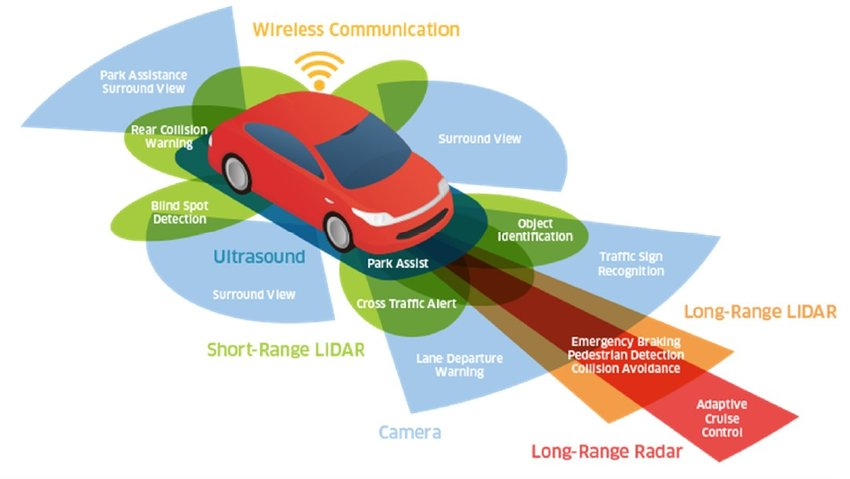
\includegraphics[width=9cm]{SensorsScheme.png}
\caption{Sensors coverage diagram for an autonomous vehicle}
{Source: }
\label{fig:p_sensors}
\end{figure*}

\subsection{Cameras}
\indent Cameras can be perceived as the most basic type of sensors that can be implemented into an AV since they are the most affordable and offer great usability. Their key role is to detect objects such as lanes, traffic signs and lights, and pedestrians to name a few. They provide readily interpretable 2D \textbf{visual} data that can span from a few centimeters to up to 100 meters. Images captured by cameras are composed of tiny elements known as pixels, which represent a specific color. Every pixel in an image collectively carries an array of pixels that form that image. 
\par The downside of cameras is that their imaging quality can significantly deteriorate in instances of bad weather, such as fog, rain and snow, and low lighting. Moreover, the amount of data output generated by cameras is immense. A single camera can generate between 20-40 MB/s on average. \cite{functionalarch}\cite{computerarch}\cite{stateoftheart}

\subsection{Radar}
\indent Radio Detection and Ranging, or radar, is a type of sensor that acts as the ultimate barrier for obstacle detection. These sophisticated systems use electromagnetic waves to detect the distance, speed, and angle of objects in the environment. We divide them into short-range, medium-range, and long-range radars, each having different applications and performance. "For 24-GHz radar, the maximum detection range is 70 m, while the maximum range increases to 200 m for 77-GHz radar."\cite{stateoftheart}[p.~6] 
\par Its primary role is to immediately react to a detected object within a dangerously close range and avoid the impending obstacle or stop the vehicle. In contrast to cameras, radars have very impressive sensing capabilities such as velocity detection, visual obstruction identification and obstacle distance measurements. It's good to mention that their data generation is significantly lower, only producing 10-100 KB/s each. On the other hand, their performance varies with signal interference, they possess low data resolution and poor color detection, and bad object classification. \cite{computerarch}\cite{Sensorfusion}\cite{stateoftheart}

\subsection{LiDAR}
\indent Light Detection and Ranging, or LiDAR, is a type of sensor that is quite similar to radar, but instead of electromagnetic waves, it uses lasers to precisely measure distance, monitor the environment and is used for mapping. It measures it by assessing the brightness of targets using pulsed laser beams from the laser emitter and analyzes the reflected light pulses with a laser receiver to create a high-definition 360-degree 3D map of the surrounding area while moving, making it a perfect tool for detecting stationary and moving objects. The distance range can vary from several centimeters to up to 200 m, depending on the type of the system. Just like radar, it can be divided into short-range, medium-range and long-range LiDARs. 
\par Its primary role is to provide precise information for immediate decision-making, allowing the vehicle to navigate and avoid obstacles effectively. In comparison to cameras, LiDAR is somewhat similar to radar. It excels at being less affected by bad weather conditions and low-light environment while staying perfectly accurate in terms of measuring the distance. On the other, compared to both of its counterparts, it's relatively expensive. "According to [\cite{stateoftheart}, p.4, in \cite{lidar}], 16
lines Velodyne LiDAR costs almost \$8000, while the Velodyne VLS-128E costs over \$100 000." On top of that, the amount of data that, the amount of data that is generated can be around 10-70 MB/s, which places a significant processing load on the computing platform.
\cite{AIandIoT}\cite{computerarch}\cite{stateoftheart}


\subsection{Ultrasonic sensors}
\indent Ultrasonic sensor is a type of sensor that utilizes high-frequency sound waves that measure the distance to the vehicle or an object. Their role is to provide accurate distance information in short-range applications, particularly for parking assistance and collision avoidance. For this reason, short-range ultrasonic sensors with 20 m detection range are employed. They are usually not used for longer ranges than that. That's where radar and LiDAR are used. 
\par In the case of data generation, it is comparable to that of radar, at around 10-100 KB/s and is quite robust in the situations of bad weather conditions and low-light environments. Moreover, they're a lot cheaper than their counterparts, given the prices are consistently below \$100. However, it's clear to see why that is since their maximum detection range is limited.
\cite{stateoftheart}\cite{Sensorfusion}

\subsection{GPS}
\indent Besides perception, navigation and guidance are essential for an autonomous vehicle. In order for the vehicle to navigate along its intended path, it needs to absorb a lot of road information in great detail, from big things like pedestrian proximity and active traffic to small ones like lane dimensions and curb heights. Based on the travel length, storing this data requires substantial memory and processing power.
\par Therefore, a Global Positioning System, or GPS, is used. GPS offers comprehensive navigation features that play a crucial role in creating a time-based route from the current position to the destination. The system must adapt to sudden path changes in order to follow the given route. It's praised for its accuracy and adaptability since it continuously redirects its route when unforeseen events, like roadblocks, are present. 
\par Although GPS's accuracy is perfect, its range is only up to 3 m depending on the circumstances, so its efficiency greatly reduces while being in closed environments, like tunnels, where satellite signals are obstructed. In such scenarios, inertial guidance using gyroscopes and accelerometers (IMU) can be a substitution to GPS.
\cite{researchresults}\cite{Sensorfusion}\cite{stateoftheart}

%nova sekcia

\section{Algorithms and techniques of data processing} \label{algorithms}

In the previous section~\eqref{sensors}, we have talked about the most important sensors of AV. The ability to process and interpret data in real-time is crucial for any AV. Hence, the true power behind these sensors comes from the algorithms that are implemented into them and the AVs in general.  

\subsection{Machine learning and deep learning}
\indent 



%zatial som toto nerozpracoval do podrobna ale zatial by som vyuzil info z \cite{stateoftheart}\cite{Sensorfusion}\cite{Taskoffloading}
\subsection{Algorithms}
\indent Since we've discussed how the sensory part of an AV works in~\ref{sensors}, we need to take a closer look on how the vehicle perceives and makes decisions of its tasks. The vehicles has the ability to process volumes of data from various sensors and simultaneously facilitate real-time decisions in order to properly function. Here we list the most important ones:

\subsubsection{Mapping}
\indent Mapping is the building block of AV's tasking. It's the process of the AV collecting data from its surroundings and creating either an image (2D) or point-cloud (3D) map of it. It's done in advance or during the making phase while employing all sensors on the vehicle. We can divide mapping into 3 modules based on its surroundings.\\
\indent \textbf{Mapping of objects} - this module compiles data received from sensors, mainly camera, radar, and LiDAR, and integrates the received information to create a 2D map. It writes down every object detected. The further ones away from the vehicles are usually collected by radar and the ones closer by the camera.\\
\indent \textbf{Mapping of the road} - this module utilizes images to establish and update the 2D map to describe the road and non-drivable surroundings.\\
\indent \textbf{Mapping traffic of regulations} - this module gathers information to create a 3D map from a LiDAR sensor containing labelled traffic signs, road markings and the positions of traffic lights.  
\cite{stateoftheart}\cite{functionalarch}

\subsubsection{Localization}
\indent Localization plays a key role in autonomous driving. It requires the integration of data gathered from various sensors, of which GPS and LiDAR systems are used the most, in order to generate a high-precision map and transfer the collected data to pinpoint the precise location of the vehicles. Therefore, the AVs can link sensor measurements together with map data for greater accuracy, which has been proven to be effective in urban environments. 
\cite{approach}\cite{computerarch}

\subsubsection{Object detection and tracking}
\indent Object detection and tracking are crucial components of AV technology since their task is to identify and monitor objects like other vehicles, pedestrians,... to ensure a safe and lawful operation of the AV. 
\par Object detection is a critical task focused on identifying vehicles, pedestrians, traffic signals/lights, and so on. Therefore, it's primarily concentrated on moving objects. The integration of point-cloud data from LiDAR sensors gains a better look at the environment while employing sensor fusion~\ref{fusion} to it as well. If shadows, identical objects and various lighting conditions are a problem for detecting an object, other sensors take place for action. The combination of a 3D map with the vehicle's position enables targeted processing which reduces both processing time and the probability of false detections.
\par Object tracking is centered on the automatic tracking of dynamic objects and ensuring safe vehicle operation/avoiding collisions with other vehicles or pedestrians. For tracking, LiDAR is primarily used since it has the ability of 360-degree vision and monitor objects over large distance in great detail. It tracks every move on the road, whether it be speeding, braking, lane changing or maneuvering. Some vehicles use two special filters for handling diverse tracking scenarios.\\
\indent \textbf{Kalman Filters} - this one is used for simple, linear tracking in scenarios where there is no change of action, for ex. constant vehicle speed, straight roads,...\\
\indent \textbf{Particle Filters} - this one is used for more complex, non-linear tracking in scenarios where there is change of action, for ex. changing speed, curved roads,...
\cite{stateoftheart}\cite{approach}

\subsubsection{Decision-making}
\indent Decision-making is central part of the AV's tasking process. It combines all of the aforementioned algorithms together to formulate a plan in order to input its driving decisions. Challenges arise from uncertain environmental factors, such as sensory data noise, unpredictable behavior, and the hidden state of other vehicles, that might damper the effectiveness of the vehicle. We divide it into 3 tasks:\\
\indent \textbf{Prediction} - AVs face a challenge when it comes to the behavior of the environment. To ensure the safe navigation of the vehicle in complex scenarios, like intersections, the AVs must possess the capability to anticipate and predict the actions of other vehicles, pedestrians on the crosswalk, and so on. One methods is creating a model that represents the positions of other vehicles and associating them with probability distributions. Therefore, AVs need perfect information about its surroundings especially with minimal dalays.\\
\indent \textbf{Path planning} - planning a path with the intention to find the safest and the most convenient way to reach a certain destination in a dynamic environment can become a challenge for an AV, the vehicles needs to employ its full maneuvering capabilities. The path planning control strategy revolves around the task of determining a geometric path from an initial configuration to the target one, ensuring the usefulness of each configuration along its path when time becomes the factor. It integrates extensive data from its system, and continuously learns and adapts so that the AV could refine its path planning strategies based on the gathered information which ultimately leads to improved decision-making.\\
\indent \textbf{Obstacle avoidance} - as safety is one of the main concerns in autonomous driving, avoiding collisions and other potential risks is a must for every AV. This algorithm operates on two levels of obstacle avoidance. The first one being the proactive mechanism which is based on the traffic predictions. During its process, it calculates certain parameters like time to collision or predicted minimum distance which is then adjusted to the local path planning. If the proactive mechanism isn't efficient enough, a second level called reactive mechanism gets active. Unlike the previous one, it relies on radar data to identify obstacles and avoid them. 
\cite{computerarch}\cite{AIandIoT}\cite{approach}

\par These components collectively form the basis for AVs to navigate through their surroundings and make informed decisions while ensuring the safety and efficiency in their operations.

\begin{figure*}
\centering
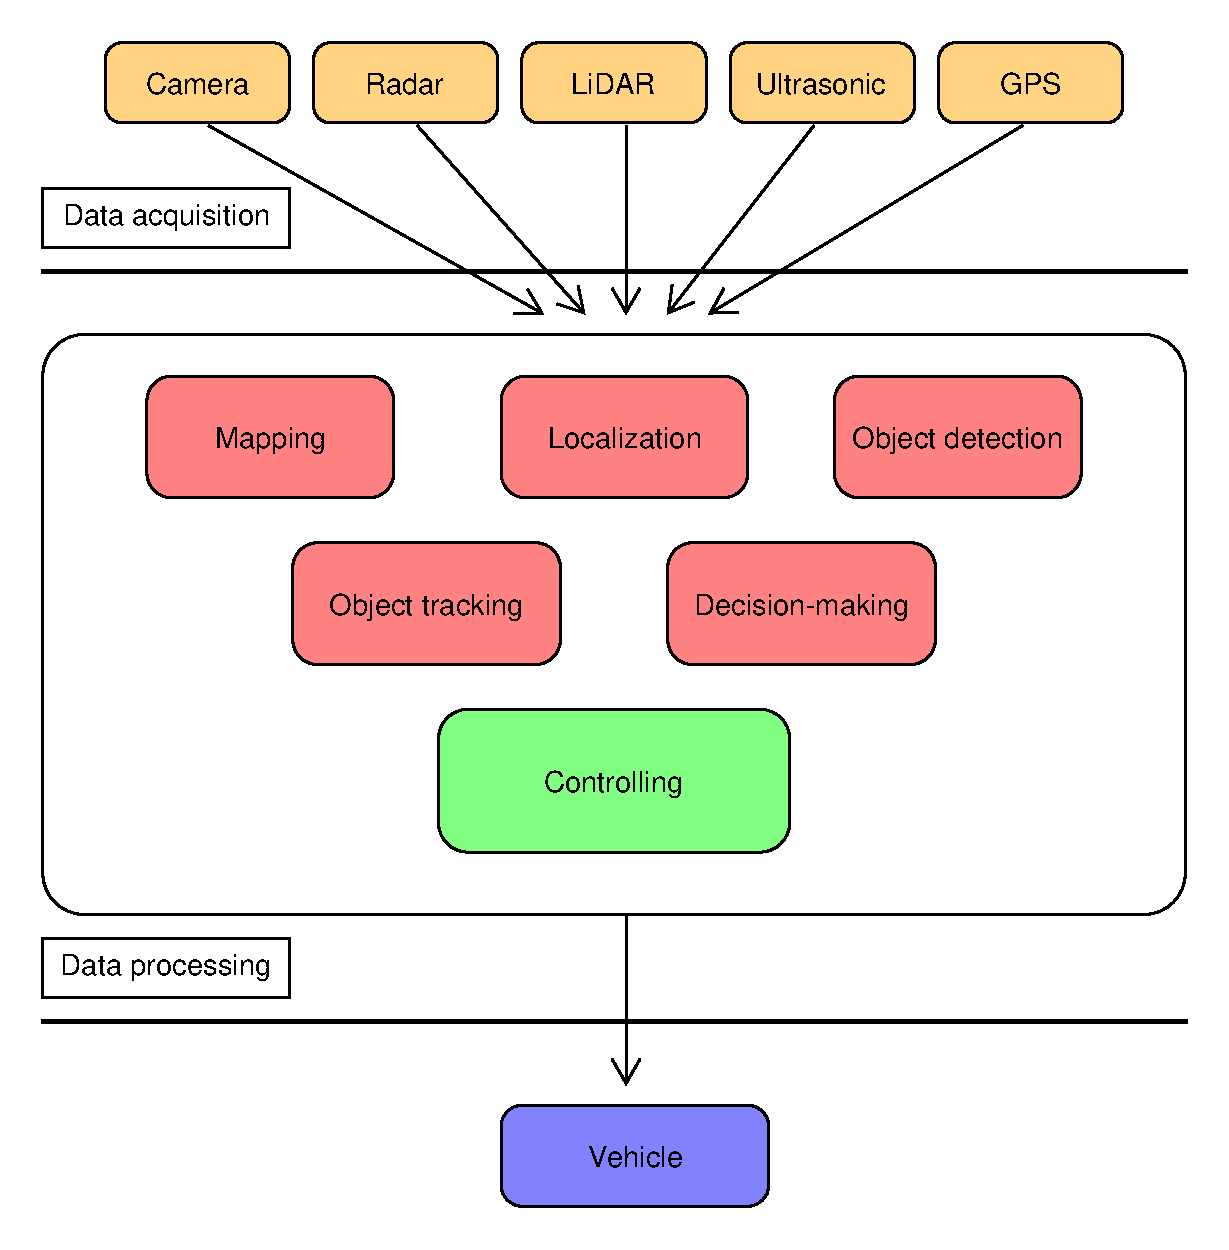
\includegraphics[width=8cm]{algoritmy.pdf}
\caption{Scheme of data acquisition and processing into the vehicle}
{Source: https://www.umlet.com/}\\
{Author: Maksim Alehash}
\label{fig:p_algoritmy}
\end{figure*}

\subsection{Sensor (data) fusion} \label{fusion}

\indent Sensor fusion is the prevalent approach that involves gathering of data from various sensors to support accurate decision-making. This mechanism unites various sensors to create a thorough perspective of the data they sense, to combine the information from these sensors, and to enhance the performance of specific detection tasks in general. With the implementation of object detection techniques based on sensor fusion, this technique offers enhanced precision when compared to the traditional object detection methods. It also aims to accurately determine the vehicle's position and orientation by combining data from these sensors. We usually divide sensor fusion framework into 5 levels:\\
\indent \textbf{1st level or level 0} - at this level, sensor fusion involves wide and narrow-band digital signal processing and automated fusion extraction methods to assess and analyze objects initially. The process helps in gathering essential information about the detected objects.\\
\indent \textbf{2nd level or level 1} - the process here relies on a more in-depth analysis and understanding of the objects detected by sensors. It combines image and non-image data sources, identifies objects through a combination of various techniques, unifies data from various sources, and adjusts the level of detail and accuracy needed.\\ 
\indent \textbf{3rd and 4th level or level 3 and 4} - the focus of this process is the assessment of the current situation and understanding its potential impact. It deals with uncertainties of various data reliability, applies automated knowledge representation and cognitive principles to make informed decision for the vehicle.\\
\indent \textbf{5th level or level 4} - the last process delves into enhancing the performance of sensors by combining them to work more efficiently and effectively, creating a well-coordinated link between sensor settings and decision-making requirements, and settings up a robust measurement to evaluate the performance and effectiveness of the entire sensor fusion system. The most common measures are Measures of Effectiveness (MOE) and Measures of Performance (MOP), which basically assess how well the system is achieving its objectives and provides improvements if needed.
\cite{AIandIoT}\cite{stateoftheart}\cite{Sensorfusion}





\section{Data processing architecture} \label{architecture}

\subsection{Edge vs cloud computing}

\subsection{vehicle communication}

\subsection{Accelarators}




\section{Safety measures and performance} \label{safety}

\subsection{Security issues}

\subsection{Security threats}


\section{Future directions and challenges} \label{future}




\section{Conclusion} \label{conclusion}



%\acknowledgement{Ak niekomu chcete poďakovať\ldots}


% týmto sa generuje zoznam literatúry z obsahu súboru literatura.bib podľa toho, na čo sa v článku odkazujete
\newpage
\bibliography{literatura}
\bibliographystyle{abbrv} % prípadne alpha, abbrv alebo hociktorý iný
\end{document}






